%%% Fiktivní kapitola s instrukcemi k PDF/A

\chapter{Výsledky}

Díky programu popsanému v předchozí kapitole bylo možné zkusit dokončit důkaz věty \eqref{veta02:hypoteza} pro některé neutrální posloupnosti $q$ (na volbě posloupnosti $p$ nezáleží, protože konstrukce pro jádrový triark nezávisí na velikosti jádra). 

Vzhledem k výpočetním omezením programu jsme zkusili dokončit důkaz věty pouze pro takové neutrální posloupnosti $q$, že $Q = {r, s}$ a navíc $r<s<18$. Seznam posloupností, pro které program nalezl potřebné grafy je v tabulce \ref{obr03:tabvysledky}. Pokud bychom se omezili na rozsah $r<s<14$, pak program grafy nalezl právě tehdy, když $r$ a $s$ jsou nesoudělná čísla.

\begin{figure}[h]\centering
\begin{tabular}{ c c c c c c c c c c c c }
  - & 7 & 8 & 9 & 10 & 11 & 12 & 13 & 14 & 15 & 16 & 17 \\
  3 & $\bullet$ & $\bullet$ &  & $\bullet$ & $\bullet$ &  & $\bullet$ & $\bullet$ &  & $\bullet$ & $\bullet$ \\
  4 & $\bullet$ &  & $\bullet$ &  & $\bullet$ &  & $\bullet$ &  & $\bullet$ \\
  5 & $\bullet$ & $\bullet$ & $\bullet$ &  & $\bullet$ & $\bullet$ & $\bullet$  
\end{tabular}
\caption{Úplný výčet dvojic stran, pro které se podařilo dokončit důkaz věty \eqref{veta02:hypoteza}.}
\label{obr03:tabvysledky}
\end{figure}
TODO označneí

Všechny potřebné grafy pro doložení důkazu jsou k práci přiloženy. TODO přiložit

Přirozenou snahou při zkoumání nalezených grafů je grafy zobrazit, aby byly pro člověka dobře čitelné. V další sekci se tomuto tématu krátce věnujeme. 

\section{Kreslení}

Přirozenou snahou pro studování nalezených grafů, a pochopení, proč právě soudělnost velikosti stěn zabraňuje v použití navrženého algoritmu k dokončení důkazu, je jejich zobrazení, které je pro člověka dostatečně čitelné. Překvapivě, i přes rovinnost grafů a celkem dobré znalosti jejich struktury není jednoduché hezké rovinné nakreslení najít.

Zamysleme se, jak graf bude vypadat. Vrcholy vnější stěny rozmístěme po kružnici a pak - podle jednotlivých hranic, které graf řeší - vždy vrcholy nově uzavřené stěny nakresleme na soustřednou, menší kružnici tak, aby spojnice žádného bodu hranice se středem kružnic neprotínala jiný bod hranice. Tímto způsobem určitě získáme rovinné nakreslení (ale hrany mohou být libovolné křivky), protože v každém kroku je možné spojit libovolné dva vrcholy, které mohou být v řešení zrovna spojovány, tak, abychom zachovali požadovanou vlastnost tvaru hranice.

Problémem takového nakreslení je počet soustředných kružnic, které bychom potřebovali, který odpovídá počtu stěn grafu. Množství potřebných kružnic by šlo celkem jednoduše snížit. Nově přidávané vrcholy nakreslíme vždy na největší kružnici, na které v příslušné výseči ještě žádný vrchol neleží. Dalším problémem by bylo rozložení vrcholů do výsečí. Představme si třeba zadání, ve kterém značný podíl tvoří souvislá posloupnost \uv{out} vrcholů. Pokud ve výpočtu dojde k uzavření stěny, která tyto vrcholy obsahuje, až na závěr, bude výseč, ve které leží, jinak zcela prázdná.

Další možností jsou běžně dostupné program či funkce na kreslení grafů. Posouzení jejich kvality na nalezených grafech necháváme na čtenáři.

Nejuspokojivější nalezenou možností je Tuttův (barycentrický) algoritmus \cite{Tutte}. Jak název napovídá, jde o umisťování vrcholů do \uv{těžišť}. Nejprve je třeba rozdělit vrcholy do dvou skupin: pevné a volné. Pevné vrcholy jsou rozestaveny, aby tvořily konvexní n-úhelník. Pozice volných vrcholů se pak dopočítá jako vážený průměr sousedních vrcholů, tedy stačí řešit soustavu lineárních rovnic.

Aby mohl algoritmus dobře fungovat, je nutné, aby graf byl 3-souvislý. Pokud by nebyl, pak vrcholy komponenty, která by po odebrání dvou vrcholů byla oddělena od zbytku grafu a neobsahovala by pevné vrcholy, budou ležet v jedné přímce.

Pro převedení grafu na 3-souvislý stačí do každé vnitřní stěny vložit vrchol a spojit ho se všemi vrcholy dané stěny. Ze způsobu, kterým graf vzniká, víme, že je 2-souvislý. Uvažujme nyní situaci po odebrání dvou vrcholů, které způsobí rozpadnutí grafu na více komponent. V každé nově vzniklé komponentě je vrchol, který je nově ve \uv{vnější stěně}. To znamená, že po přidání vrcholů pro stěny bude jedním z nich spojen s další komponentou a tedy bude 3-souvislý. 

V našem případě za pevné vrcholy volíme vrcholy vnější stěny, které jsou rozmístěné na kružnici a podle konkrétního grafu je pak možné nastavit váhy jednotlivých vrcholů. Obecně se pro dostatečně malé grafy (do 40-ti vrcholů) osvědčila lineární závislost váhy na pořadí přidání vrcholu do grafu, nejdříve přidaný je nejtěžší.



\begin{figure}[h]\centering
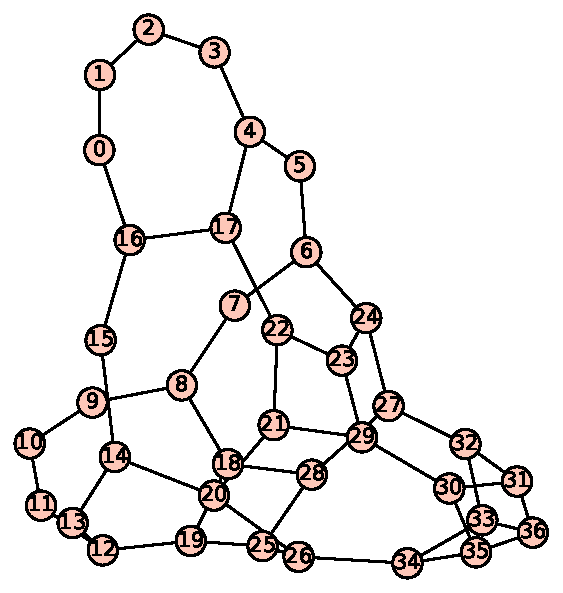
\includegraphics[width = 60mm]{../img/sageplot}
\caption{Automatické nakreslení SageMath.}
\label{obr03:konstrukceiv}
\end{figure}


\begin{figure}[h]\centering
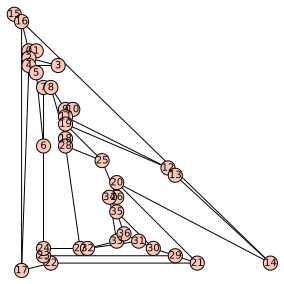
\includegraphics[width = 60mm]{../img/planar}
\caption{Rovinné nakreslení SageMath.}
\label{obr03:konstrukceiv}
\end{figure}


\begin{figure}[h]\centering
\includegraphics[width = 60mm]{../img/Triarc15150{4,7}__v37}
\caption{Neato s předdefinovanými pozicemi vnější stěny.}
\label{obr03:konstrukceiv}
\end{figure}


\begin{figure}[h]\centering
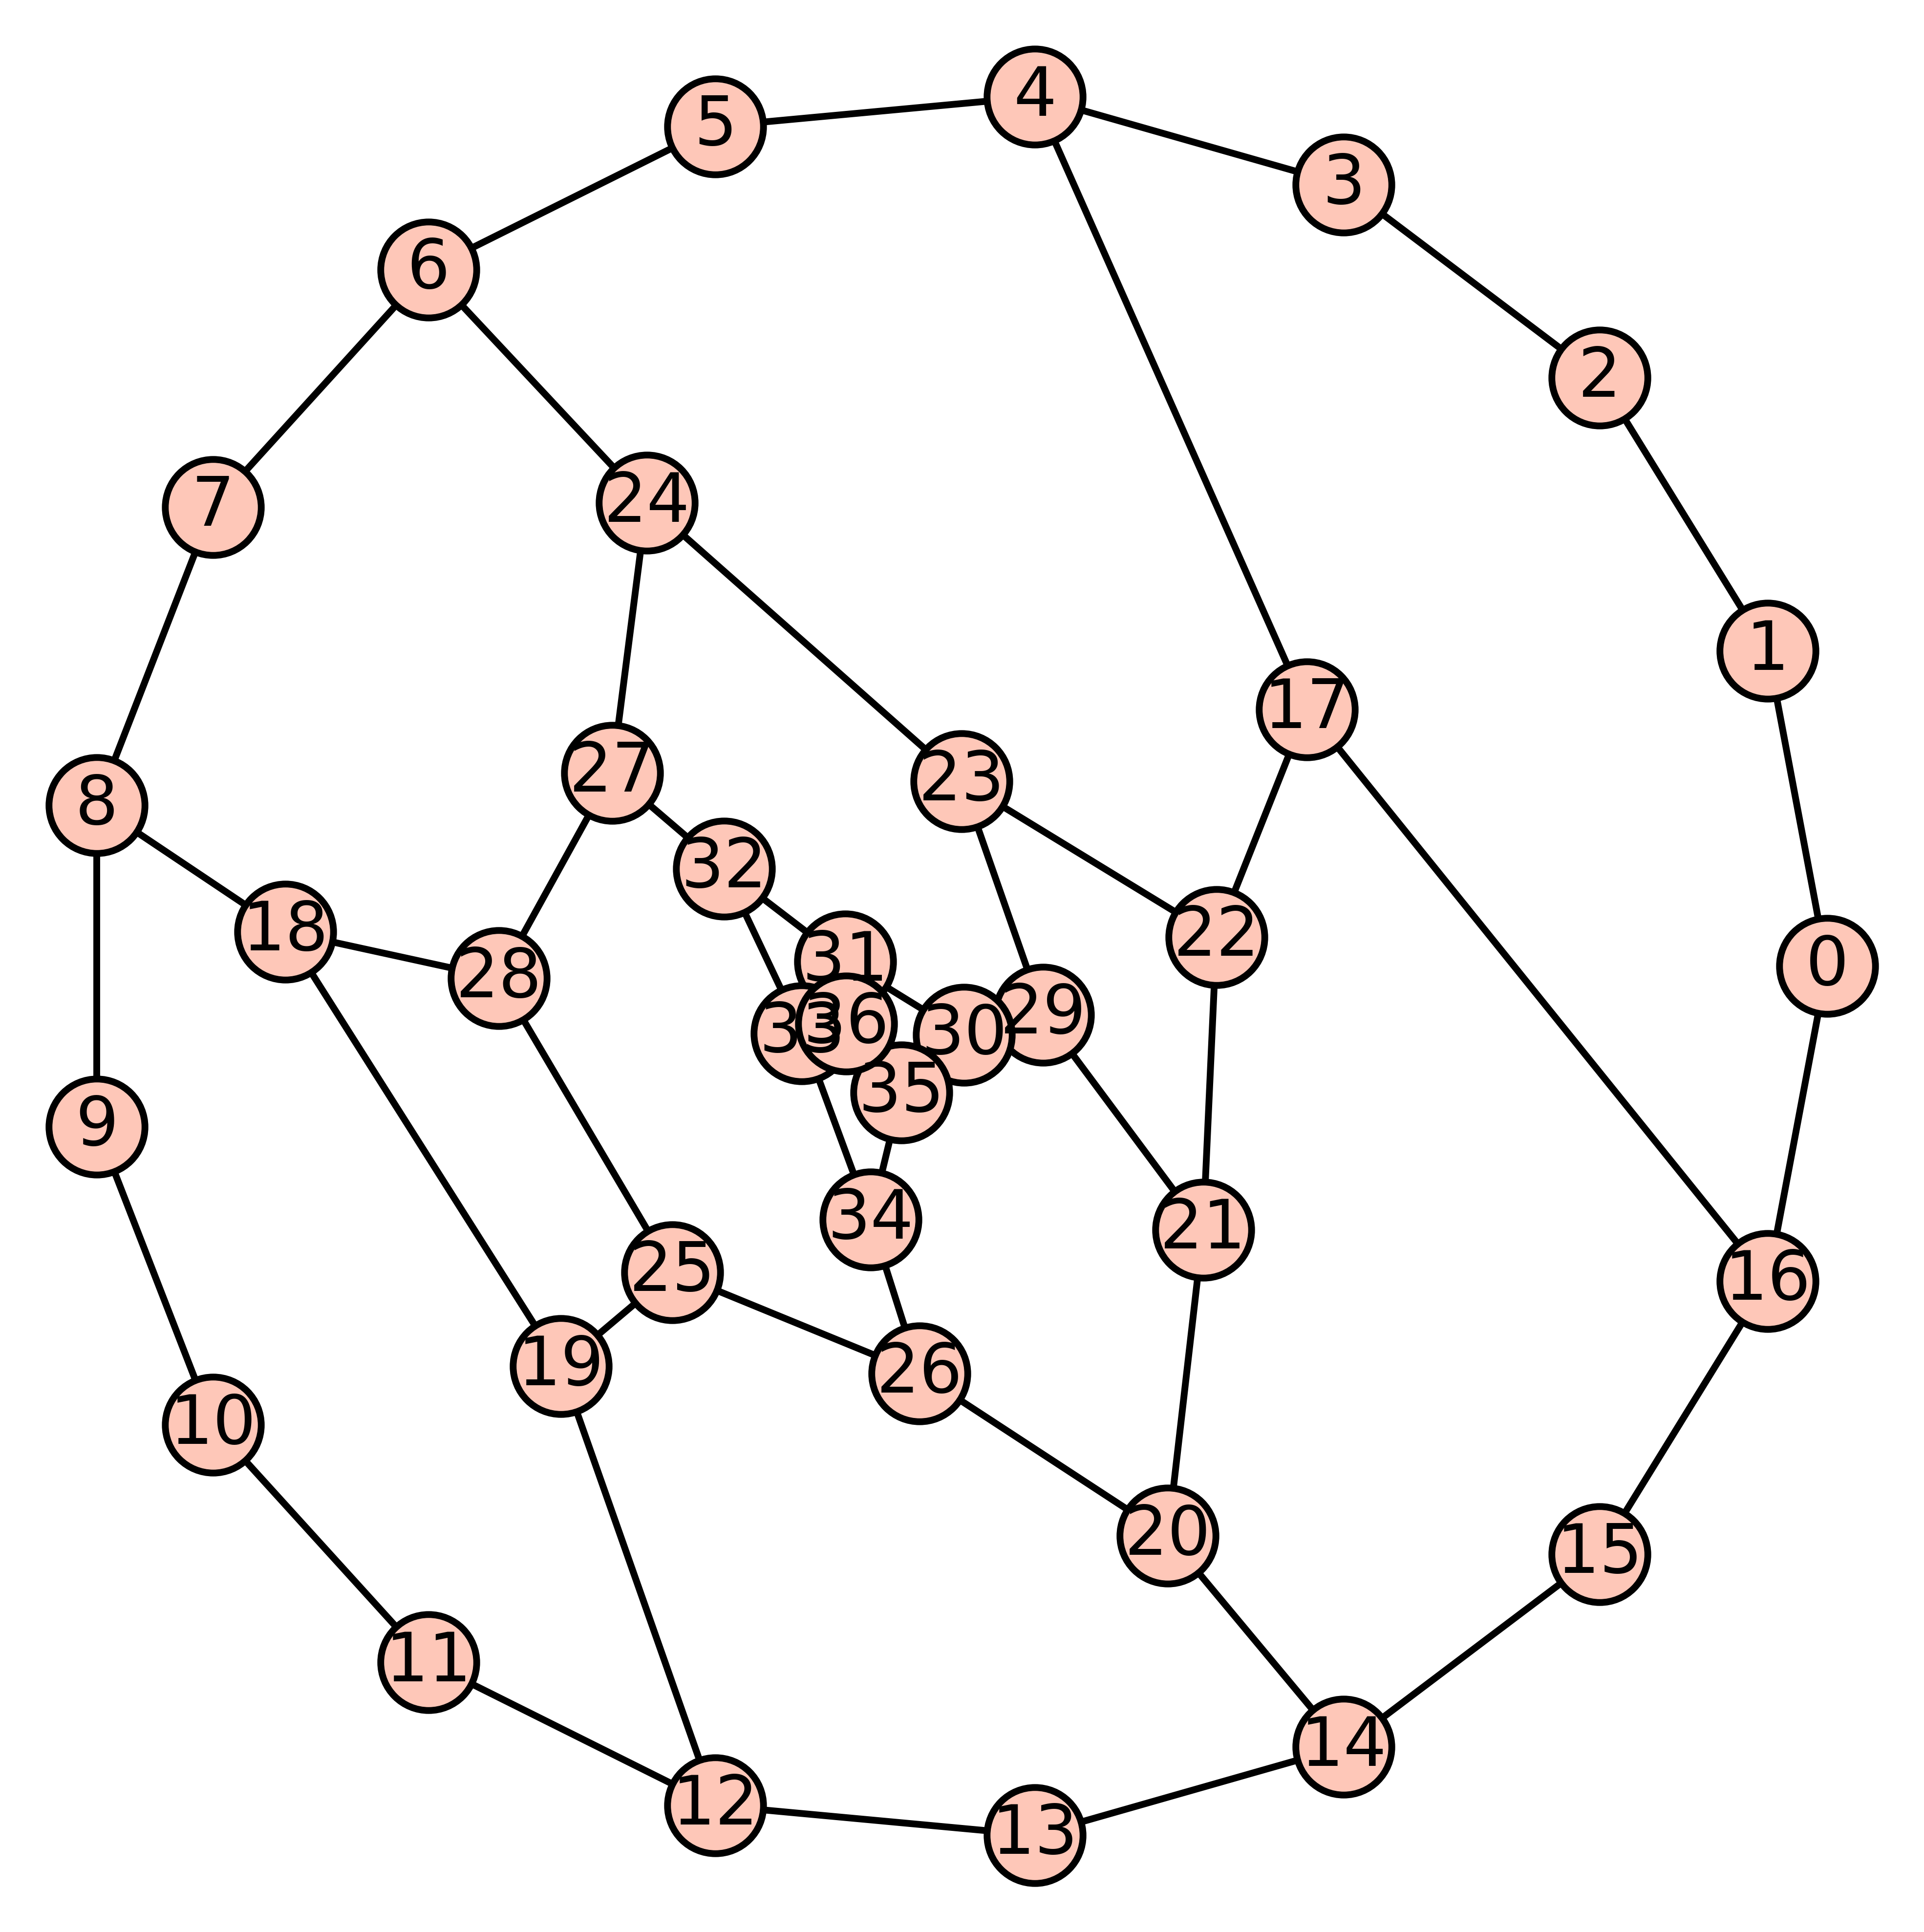
\includegraphics[width = 60mm]{../img/tutteplot}
\caption{Tuttovo nakreslení.}
\label{obr03:konstrukceiv}
\end{figure}



Při hledání triarků byla vynaložena netriviální snaha pro nalezení způsobu, jak výsledný graf dobře zobrazit - od rovinného grafu by se dalo čekat, že nepůjde o příliš složitý úkol. Po špatné zkušenosti s dostupnými možnostmi jako GraphViz nebo funkcemi v SageMath, došlo na implementaci kreslícího algoritmu založeného na Tuttově kreslení TODO zmínit odkaz a dál o kreslení nemluvit? Nebo popsat? 
